% Copyright (c) 2005, 2006, 2007, 2008, 2009 Center for Urban Simulation and Policy Analysis,
% University of Washington.  Permission is granted to copy, distribute and/or
% modify this document under the terms of the GNU Free Documentation License,
% Version 1.2 or any later version published by the Free Software Foundation;
% with no Invariant Sections, no Front-Cover Texts, and no Back-Cover Texts.
% A copy of the license is included in the section entitled "GNU Free
% Documentation License".

\documentclass{howto}  
\usepackage{graphicx, html}
\usepackage[T1]{fontenc}

\begin{document}

\newcommand{\package}[1]{\index{opus packages!#1@\textit{#1} package} \textit{#1}}


\title{How to Generate a Lorenz Curve\\and Gini Coefficient}

%\release{0.1}

\author{Center for Urban Simulation and Policy Analysis\\
University of Washington}

\authoraddress{Daniel J. Evans School of Public Affairs \\
University of Washington \\
Seattle, Washington 98195 \\
USA \\
% Put the real email address only in the pdf version (to avoid including
% a spam magnet in the html version).  A mangled version of the address
% (using "info (at) urbansim.org") is included in the html version by
% a parameter to the latex2html command
%begin{latexonly}
Email: \email{info@urbansim.org} \\
Web Site: \url{www.urbansim.org}
%end{latexonly}
}

%\date{\today}
% replace \today with a real date (\date{April 1, 2000} ...} when this
% manual is ready for release so that reformatting doesn't cause a
% new date to be used.  For now, setting the date to \today during
% early editing makes it easier to handle versions.

\maketitle

\section{Introduction}

This tutorial describes two measures of inequality available in UrbanSim
(the Lorenz curve and Gini coefficient), and how to generate them using the
Opus indicator maker.

The Lorenz curve indicator in available in UrbanSim as a visual
representation of the distribution of a non-aggregate variable over the
population.  It is used to examine the fairness with which impacts
(benefits and costs) are distributed in a given scenario.  The Lorenz curve
is a graph which represents the cumulative distribution function of a
probability function over a population.  It is commonly used in the
analysis of inequality.  The Lorenz curve allows flexible analysis of
equity because it is not limited to a specific type of population or
variable that is distributed among that population.  The Gini coefficient
is another way to measure equity, and is derived from the Lorenz curve.
 

Flexible equity analysis is important for many reasons.  
\begin{enumerate}
\item There are different ways to look at equity, such as fairness or social justice.
\item There are different ways to categorize people for equity analysis, including location, age, income, family status, pedestrians, etc.
\item There are different ways to measure an impact on a group.  For example  noise, pollution, land value, income and access to transportation can all be affected by a policy.  
\item There are different types of equity, and they can overlap and conflict with one another.  For example a policy that ensures fairness (everyone is treated the same) may not take into account that different groups have different needs. 
\item Stakeholders' values can vary and change with time. 
\end{enumerate}

This tutorial covers creating an indicator with a Lorenz curve selected as the visual output.  The specific properties of the Lorenz curve and the Gini coefficient are discussed as well as their common applications and limitations. 

\section{The Lorenz Curve}

\begin{figure}
\begin{center}
%begin{latexonly}
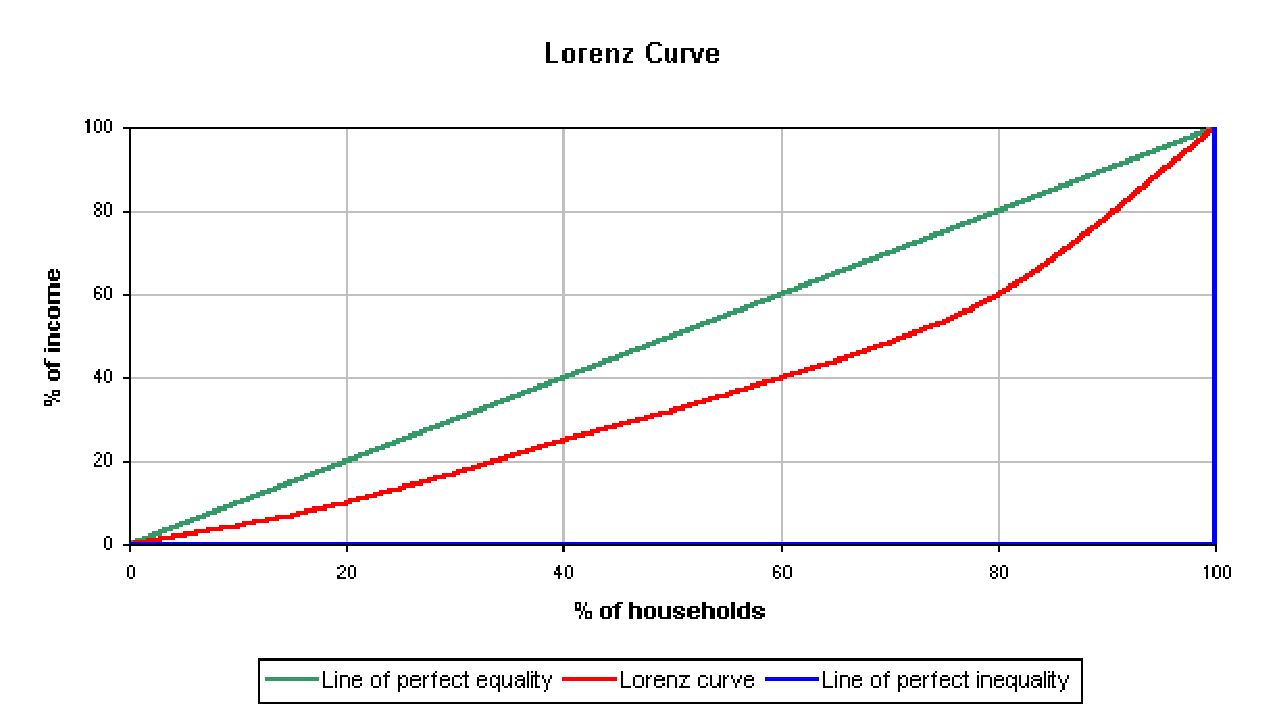
\includegraphics[width=150mm]{images/Lorenz.pdf}
%end{latexonly}
\caption{Lorenz Curve Example}
\htmlonly{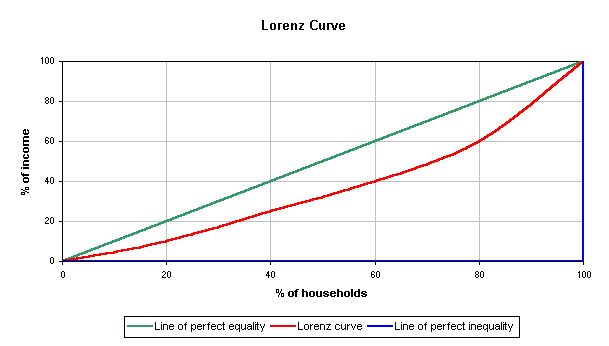
\includegraphics{images/Lorenz.jpg}}
\end{center}
\end{figure}

In this example, the population is represented as households and plotted on the x axis from 0\% to 100\%, and the variable income, is plotted on the y axis, also from 0\% to 100\%.  The line of perfect equality is the baseline function, and displayed in this figure as the green line.  The red curve is composed of discrete points because the amount of data is finite. In cases where the curve does not lie on the line of perfect equality, every point on the curve represents a 
statement like: "the bottom 20\% of households has 10\% of the total income".

The Lorenz curve can be represented by a function $L(F)$, where $F$ is the horizontal axis, 
and $L$ is the vertical axis.

For a population of size n, with a sequence of values $y_{i}$ $i = 1$ to $n$ that are indexed in non-decreasing order $(y_{i} <= y_{i+1})$ the Lorenz curve is the continuous piecewise linear function connecting the points $( F_{i} , L_{i} )$, $i = 0$ to $n$, where $F_{0} = 0, L_{0} = 0$, and for $i = 1$ to $n$: \\

    $F_{i} = i/n \\
    S_{i} = \Sigma_{j=1}^i \; y_{j} \\
    L_{i} = S_{i} / S_{n}$ \\

The amount of inequality in two societies, or in two scenarios can be compared
based on their Lorenz curves.  If the curve in one case is farther away from
the line of perfect equality for every value along the horizontal axis, then
that case is considered to have less equality than a case with a curve nearer
to the equality line.

The line of perfect equality in the Lorenz curve is $L(F) = F$ and represents a uniform distribution, or equality.  

Properties: \begin{enumerate}
\item A Lorenz curve always starts at (0,0) and ends at (1,1).
\item The Lorenz curve is not defined if the mean of the probability distribution is zero or infinite.
\item The Lorenz curve for a probability distribution is a continuous function. 
However, Lorenz curves representing discontinuous functions can be constructed as the 
limit of Lorenz curves of probability distributions, the line of perfect inequality 
being an example.
\item Lorenz curves are scale invariant.  They do not take into account whether distributions have
different total values, rather they are based on how these values are distributed.  
\item Lorenz curves can be used to look at a distribution of a single year, or the changes in the Lorenz curve over time can by analyzed.
\item If the variable being measured cannot take negative values, the Lorenz curve: it cannot rise above the line of perfect equality, cannot sink below the line of perfect inequality, is increasing function, and is a convex function. 
\end{enumerate}

\section{The Gini Coefficient}

The Gini coefficient is a ratio of the areas on a Lorenz curve. 

\begin{figure}
\begin{center}
%begin{latexonly}
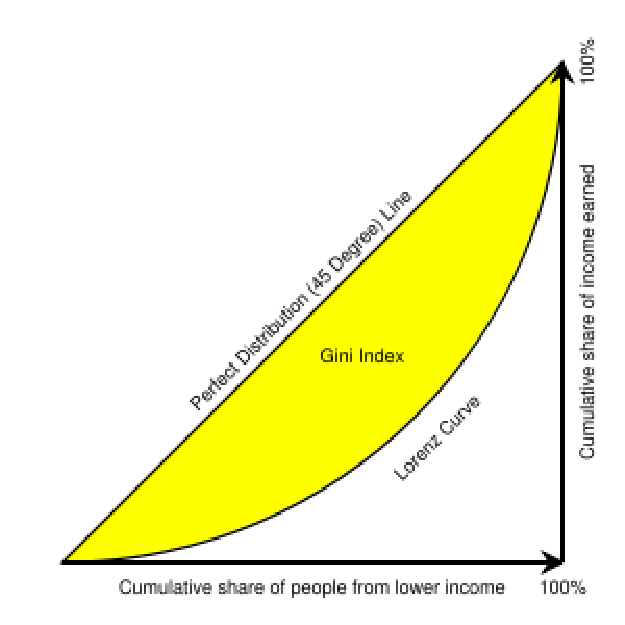
\includegraphics[width=100mm]{images/gini.pdf}
%end{latexonly}
\caption{Gini Coefficient Example}
\htmlonly{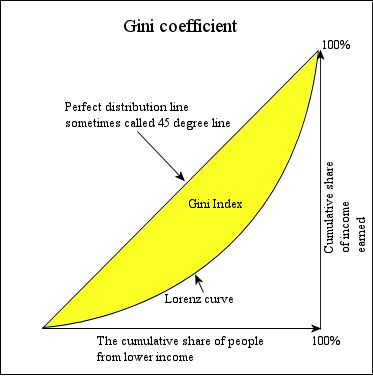
\includegraphics{images/gini.jpg}}
\end{center}
\end{figure}

It is also a measure of the inequality of a distribution.  If the area between the line of 
perfect equality and Lorenz curve is A, and the area under the Lorenz curve is B, then the 
Gini coefficient is $A/(A+B)$. Since $A+B = 0.5$, the Gini coefficient, $G = A/(.5) = 2A = 1-2B$. 
If the Lorenz curve is represented by the function $Y = L(X)$, the value of B can be found with integration and:

    $G = 1 - 2\,\int_0^1 L(X) dX$ 

Some important properties of the Gini coefficient are:
\begin{enumerate}
\item The Gini coefficient is a measure of inequality of a distribution. It is defined as a ratio with values between 0 and 1: the numerator is the area between the Lorenz curve of the distribution and the uniform (perfect) distribution line; the denominator is the area under the uniform distribution line.
\item It is often used as a metric of inequality.
\item The higher the Gini coefficient, the greater the inequality.
\item A value of zero corresponds to perfect income equality (everyone has the same income), while a value of 1 corresponds to perfect income inequality (one person has all the income, and the rest of the population has none).  
\item It is not affected by the shape of the Lorenz curve, only by the ratio of the areas used to compute it.
\item It does not indicate how the inequality is distributed, only the total amount of inequality. 
\item The Gini coefficient can be used to indicate how a distribution changes over time and if this change shows that equality is increasing or decreasing.
\end{enumerate}

\section{Meaningful Inputs}

The types of inputs that are commonly used to generate a Lorenz curve and 
Gini coefficient are non-aggregate variables. 

The most common input for the Lorenz curve and Gini coefficient is individual or household
income, because income is an important measure of well-being.  Other variables
could also be the basis for distributional comparisons.  These should be
non-categorical quantities, such as the amount of water consumed, carbon emitted, or 
taxes paid.  At a higher level of aggregation it also makes sense to consider
percentages, such as a fraction of a certain area whose residents are ethnic
minorities, voted Independent, or have incomes below poverty.  Finally, it may be
helpful to consider that the normative implication of a Gini coefficient is that perfect 
equality is preferred.  Certain variables which can be analyzed for their distribution, such as miles of light rail track,
may not necessarily be best when equally spread but rather more valuable when
grouped together in certain places.

The typical unit of analysis for a Gini coefficient is the individual.  UrbanSim allows for the use of the Gini
in assessments of equity across units such as gridcells and zones.  Parcel level
analysis will be supported in the future.  It is valid to measure distributions across 
these units, however the user should keep the units in mind when interpreting the results.

\section{Limitations}

Lorenz curve limitations:
\begin{enumerate}
\item When comparing two Lorenz curves, it is not possible to determine which distribution has more inequality if the two curves intersect. 
\item The amount of inequality may be misleading.  For example when looking at the distribution of income, the amount of inequality could be understated if richer households are able to use their incomes more efficiently than lower income households.
\item Life cycle effects are ignored. For example an individual's income varies over his lifetime, and this variation is not considered when analyzing inequality with a Lorenz curve.
\end{enumerate}

Gini coefficient limitations:
\begin{enumerate}
\item The Gini coefficient cannot be used when the values of the variable distributed among the population can take on negative values.  For example if used to look at income inequality, it must be the case that no one have a negative net wealth.
\item The measure will give different results if applied to individuals instead of households.  For comparison to be meaningful, the populations must be looked at with consistent definitions.


\end{enumerate}
These limitations help to understand the problems caused by the improper use of equality 
measures. However, they do not render these measurements ineffective. If equality measures 
are computed in a well-documented and consistent way they can provide a good tool for 
quantitative comparisons.

\section{Tutorial Prerequisites}

If you have not already done so, install the necessary software and data
for this tutorial by following the Installation Instructions at
\url{http://www.urbansim.org/download}.  This tutorial also assumes that
the user is familiar with the OPUS framework and generating indicators, or
has completed the Eugene tutorial linked from the download page.

\section{Computing an Indicator}

UrbanSim ``indicators'' are useful representations of dataset attributes.  
How these dataset attributes are displayed is specified by the user.  
In this example a Lorenz curve is generated.

\begin{enumerate}

\item In your command window, make sure you are in the
\file{eugene\textbackslash tools} directory.  Then type the following command to
open a tool that will allow us to specify and then view an
indicator:

\begin{verbatim}
python create_indicator.py
\end{verbatim}

\item In the ``Cache directory'' field, enter the location of the cache directory
created by the
simulation, e.g. \file{C:\textbackslash urbansim_cache\textbackslash
run_2006_11_15_15_12}.
This will be a directory in the output directory you specified when
starting the simulation.

\item Leave the ``Compare to another cache directory'' unchecked.  This
option lets you compare results from two different simulations, and isn't
used here.

\item Select ``Lorenz Curve'' from Type drop down menu. This automatically
generates the Gini coefficient as well.

\item In the ``Attribute'' field, enter:

\begin{verbatim}
urbansim.gridcell.average_income
\end{verbatim}

This entry contains the ``Opus path'' for a variable that shows the
average income within each gridcell.  More specifically, this Opus path specifies
the location of a Python file defining this gridcell : it is
in the \package{urbansim} Opus package, is defined for the
\verb|gridcell| dataset, and is located in the Python file named
\file{average_income.py}. You can find the file containing the \package{urbansim}
package inside your workspace directory.

\item Leave the optional ``Name'' entry empty. If entered, it is used
as the name for the created indicator (and also determines the filename of the
resulting indicator). We'll let the program use the default name
(``average_income'' in this case).

\item Type in ``gridcell'' in the ``Dataset'' entry.  This is consistent with the attribute 
we're going to create indicator for. 

\item Type in 1982 in the ``Year(s)'' entry. 

\item Press ``Run Request'' to generate this indicator.

\item The tool will then compute the indicators. When the
``View results'' button becomes active, it means the computation has finished.
Press this button. A web
browser will be launched and page loaded with a link to the requested indicator.

\item Click on the ``1982'' link to see the Lorenz curve. This simple plot was
produced by matplotlib, a Python graphing and mapping package.  


See \url{http://www.urbansim.org/wiki/external/index.php/Indicators} for an example of the partial list of indicators that are known to work on the Eugene-Springfield data.  Interpreting the Lorenz curve and Gini coefficient is defined for non-aggregate variables.  

\item Press ``Close'' to exit this tool.

\end{enumerate}

\section{Closing Comments}

At this point, you have generated a Lorenz curve and Gini coefficient 
produced by an indicator from the simulated results. 
For more information, please see the accompanying Reference Manual and User Guide. 

If you have any particular requests for documentation, let us know by emailing
the \url{users@urbansim.org} email distribution list.

\section{Acknowledgments}

This tutorial was put together by students from the 2007 UrbanSim Capstone class of the Computer
Science and Engineering department at the University of Washington
and from the Daniel J. Evans School of Public Affairs to accompany the integration
of Lorenz curve output into the OPUS core.

\section{References}
Cowell, Frank A. \emph{Measuring Inequality}. Oxford: P. Allan, (1977).

\end{document}

% LocalWords:  urbansim lorenz gini capstone dX UrbanSim gridcells dataset py


%%% Local Variables:
%%% mode: latex
%%% TeX-master: "userguide"
%%% End:
% LocalWords:  eugene gridcell filename matplotlib userguide
